\chapter{Data}

To the best of our knowledge, no publically available dataset exists with images or videos of fetuses while in pain exposure. This fact alone highlights the novelty and innovative aspects of our research, which was developed in collaboration with the study group of Fetal Pain from the University of São Paulo (USP). 

This group studies pain assessment techniques and conduct clinical trials on the topic. They were responsible for collecting the videos used in our work as well as assisting with the medical background to help answer our questions.

\section{Data Collection}

The videos were recorded from a 4-D ultrasound machine of the model Voluson E8 by General Electric. They were recorded in three groups, for a total of 15 videos, being five from each group. All the fetuses were in the third trimester of gestation, with an average of 31.1 weeks with a 2.8 standard deviation.

The first set of videos was a baseline with fetuses in resting conditions. All the recordings were made during routine exams for prenatal care.

The second group was of fetuses that had to go through intra-uterine surgery, and thus needed fetal anesthesia. For these cases, the exact moment of the anesthetic puncture was recorded to capture the reaction of the fetus and its manifestations of pain. Videos from this group had two parts in it, first a baseline period defined for the first 30 seconds before the anesthesia puncture and second the 45 seconds immediately after the puncture.

For this group, specifically, a second ultrasound machine was placed in the clinical room. While the main one was used for the medical procedure, the second targeted the fetus's face to monitor its expressions. This setup can be seen in Figure \ref{fig:ultrasound}.

\begin{figure}[h!tp]
    \centering
    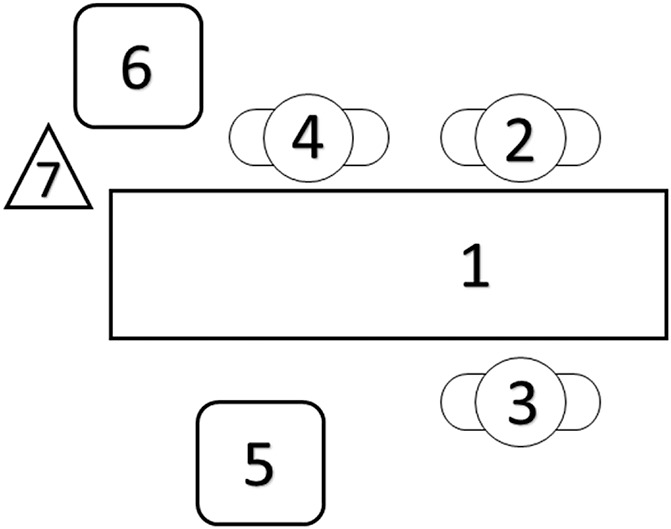
\includegraphics[width=.35\textwidth]{imgs/chap03_ultrasound_setup.jpg}
    \caption{\textcolor{red}{Dúvida: Como citar figuras de outros artigos?}}
    \label{fig:ultrasound}
\end{figure}

Lastly, the third group was recorded while the fetus was exposed to the sound of a horn, which was meant to cause distress but no harm, thus it serves as a control group from which we expect to be able to differentiate from pain.

\section{Ethics}

All mothers have given written informed consent to participate in the study and to record the behavioral reactions of the fetuses. The study was also approved by the hospital's ethics review board.

\section{Pain Evaluation}

Images from the videos were reviewed by two blinded researchers who independently scored the facial pictures of each fetus using the Neonatal Facial Coding System to quantify the amount of pain. The reviewed factors were: deepening of the nasolabial furrow, open lips, horizontal mouth stretch, vertical mouth stretch, lip purse, taut tongue, tongue protrusion, chin quiver, brow lowering, and eyes squeezed shut. They have also added two other factors: yawning and neck deflection. These factors are commonly mentioned in medicine research observations of fetal reactions after a stimulus.

